\chapter{Tag Clouds}
\label{sec:semannot}


We have found so far no other application implementing LSA in order to present an overview of the main topics found in a collection of unstructured texts, based on user queries. The TagCloud Summarizer is in this sense new.\\

There exist, however, search engines, which utilize categorizing of search results, such as Yippy(former Clusty, Vivisimo). It utilizes search, classification, and Social web (Web 2.0).
\section{existing implementations}
http://cloud.yippy.com/  - visualizes topics based on search queries. Created at Vivisimo company, also creator of one of the most successful meta search engines, offering classification of search results, Clusty (Vivisimo). \\

SenseBot Summarizer summarizes search results in the form of a tag cloud.\\

Google on the other hand offers "Wonder wheel" option, in order to display search results \\ 

TagCloud Summarizer is a tool that users can use to instantly visualize a topic using the familiar tag cloud display. Users can create a cloud based on a query.\\

TagCloud Summarizer generates a cloud using the user's search results for the topic they enter. Using the Summarizer to generate the cloud also ensures that it is always up-to-date because topics/main concepts are generated in real-time, based on the user's query.\\

\section{use}
Use the TagCloud Summarizer for online web-pages, search systems, or personal web-sites.\\

\begin{summary}
This chapter presents an overview of tagclouds used as a method for representing text content.
\end{summary}

Tag Clouds are popular applications used for vaious purposes: as a navigation mechanism, as indicators of activity within social media experiences, for visualization in texts and textual data, for annotation of documents~\ref{fig:tagcloud}. The importance or weight of words in the tag cloud are shown with size of font and/or color. The tag clouds are hyperlinks leading to a collection of items associated with the tag.\\
A version of tag cloud is called text cloud. It is used as a visual display that conveys the broad themes that emerge from textual analysis.  
There are three types of tag clouds depeding on their purpose and use. The first type contains a tag represeting the frequency of each term. The second type is a global tag cloud whose tags has frequencies aggreggated over all items and users. The third type of tag cloud contains categories, and its tags' size indicates the number of subcategories.\\
%TODO
%generate a tag cloud based on the contents in docmachine!!!!!!! replace the figure
%
% Opencloud
%
\begin{figure}[htbp]
	\centering
	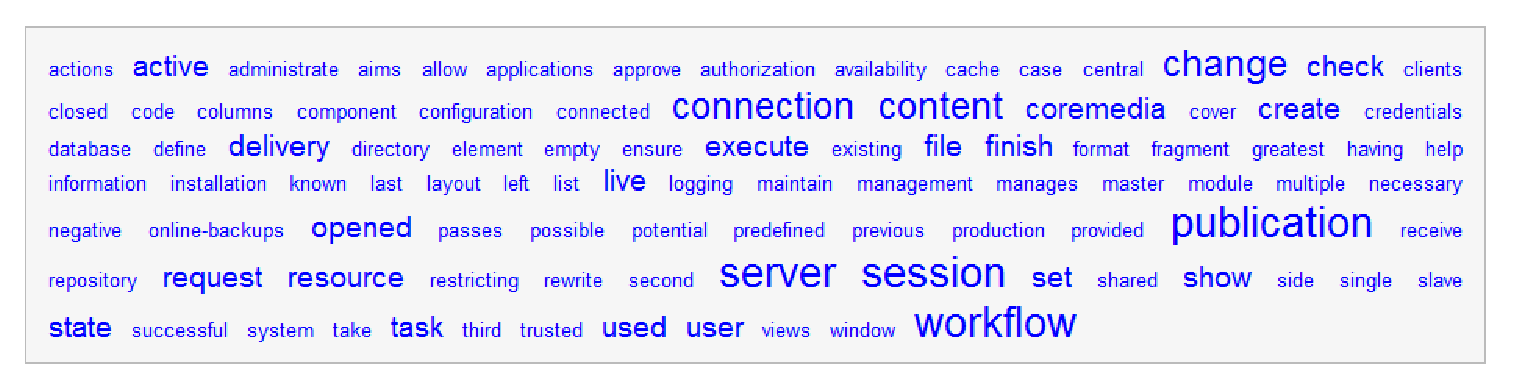
\includegraphics[width=\ScaleIfNeeded]{img/tagcloud} 
 % or [scale=0.5]
	\caption{Tag Cloud}
	\label{fig:tagcloud}
\end{figure}

\section{1}
\label{sec:semannot:1}
Related work \\
Opinion Crawl\footnote{\url{http://www.opinioncrawl.com/}} - web sentiment analysis application. It generates a concept cloud from daily scanned blogs, web site articles. \\

SenseBot Search Results Summarizer is a plugin for Mozilla Firefox browser that generates a tag cloud of the main concepts returned as search results from Google. \\

Search Cloudlet\footnote{\url{https://addons.mozilla.org/en-US/firefox/addon/9943/}} is another Firefox Addon that inserts a related tagcloud into Google interface. Working behind the scenes, Search Cloudlet injects a tag cloud of related words in to both Google and Yahoo search results pages. Then you can use the tag links to quickly and easily filter and refine your searches.



LinkSensor
SenseBotSummarizer
All three are based on SenseBot - a semantic search engine.
Made available from Semantic Firefox Extensions \footnote{\url{http://www.semanticengines.com/plugins.htm}}\\

\section{Brainstorming}
What is a tag cloud? Graphical representation of a collection of tags. Tag clouds visualize word frequency in a given text.\\

Tag clouds may be used as a topic summary.\\

There are three main types of tag cloud applications used in social software.\\
\begin{enumerate}
\item frequency of items / tags
\item number of items to which a tag has been applied
\item tags are categorization method for content items 
\end{enumerate}
The following tag clouds were evaluated in order to select the solution that is most applicable for Tag Cloud Summarizer project.\\
\begin{itemize}
\item TagsTreeMaps\footnote{\url{http://tagstreemaps.sourceforge.net/TagsTreeMaps.html}}
\item OpenCloud\footnote{\url{http://opencloud.sourceforge.net/}}
\end{itemize}
